\documentclass[../main.tex]{subfiles}

\begin{document}

\section{Matrix Multiplication}

Before we get into formulas and computations, let's build our
intuition on what a matrix and its multiplication is supposed to
represent. We will discuss \textbf{linear transformation} in
depth in latter notes, but we can think of it as a function that
transforms the vector space. Matrix instructs the function how to
transform the space. Let's take a look at a quick example.

Let $A$ be a matrix that has order $2 \times 2$. The first column
tells how to map the $\hat{i}$ and the second column represents
where our $\hat{j}$ is mapped.
\[
\begin{bmatrix}
    2 & 1 \\
    1 & 3
\end{bmatrix}
\]
Matrix $A$ is telling us to map the standard basis $\hat{i} =
\langle 1, 0 \rangle$ to $\hat{i}'= \langle 2, 1 \rangle$ and from
$\hat{j} = \langle 0, 1 \rangle$ to $\hat{j}' = \langle 1, 3 \rangle$.
Consider the diagram below.

\begin{figure}[H]
\centering
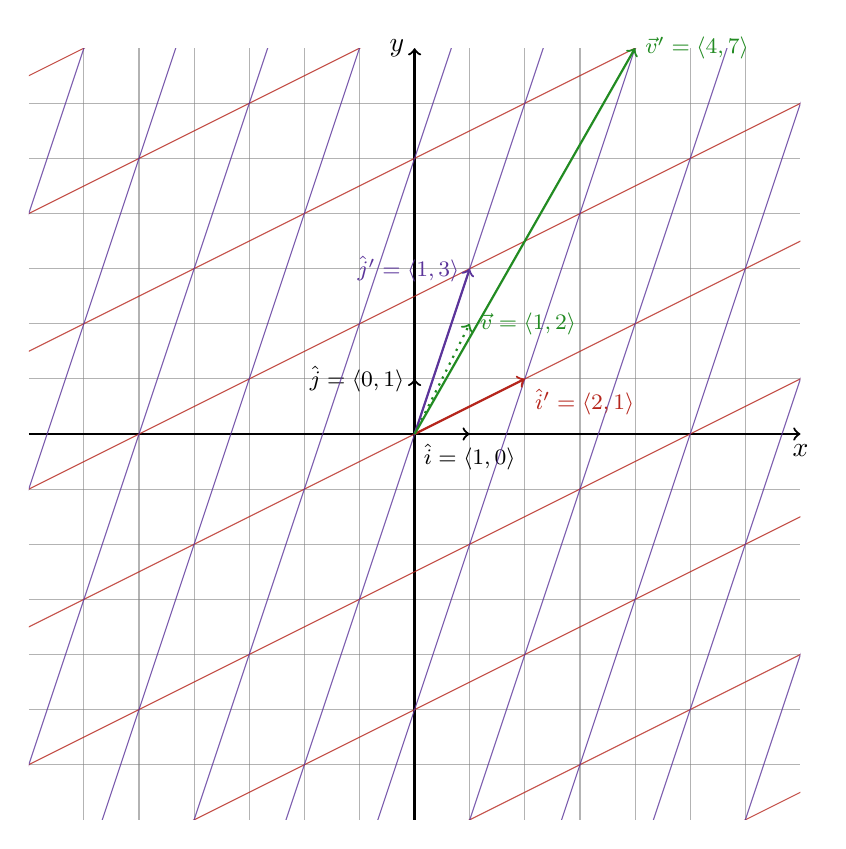
\begin{tikzpicture}[
        vector/.style={->, thick},
        scale=0.7
    ]

    \foreach \i in {-6, -5, ..., 6} {
        \draw[gray, thin, opacity=0.6] (\i, -7) -- (\i, 7);
        \draw[gray, thin, opacity=0.6] (-7, \i) -- (7, \i);
    }
    \draw[vector, black] (-7, 0) -- (7, 0) node[below] {$x$};
    \draw[vector, black] (0, -7) -- (0, 7) node[left] {$y$};

    \draw[vector] (0, 0) -- (1, 0) node[below]
        {\footnotesize $\hat{i} = \langle 1, 0 \rangle$};
    \draw[vector] (0, 0) -- (0, 1) node[left]
        {\footnotesize $\hat{j} = \langle 0, 1 \rangle$};
    \draw[vector, dotted, ForestGreen] (0, 0) -- (1, 2)
        node[right, ForestGreen]
            {\footnotesize $\vec{v} = \langle 1, 2 \rangle$};

    \begin{scope}
        \clip (-7, -7) rectangle (7, 7);

        \foreach \j in {-10, -9, ..., 10} {
            \draw[BrickRed, opacity=0.8]
                ({-10*2 + \j*1}, {-10*1 + \j*3})
                    -- ({10*2 + \j*1}, {10*1 + \j*3});
        }
        \foreach \i in {-10, -9, ..., 10} {
            \draw[RoyalPurple, opacity=0.8]
                ({\i*2 + -10*1}, {\i*1 + -10*3})
                    -- ({\i*2 + 10*1}, {\i*1 + 10*3});
        }
    \end{scope}

    \draw[vector, BrickRed] (0, 0) -- (2, 1)
        node[below right, BrickRed]
            {\footnotesize $\hat{i}' = \langle 2, 1 \rangle$};
    \draw[vector, RoyalPurple] (0, 0) -- (1, 3)
        node[left, RoyalPurple]
            {\footnotesize $\hat{j}' = \langle 1, 3 \rangle$};
    \draw[vector, ForestGreen] (0, 0) -- (4, 7)
        node[right, ForestGreen]
            {\footnotesize $\vec{v}' = \langle 4, 7 \rangle$};
\end{tikzpicture}
\end{figure}

After the transformation, you can imagine mapping everything
in the standard vector space with respect to the new colored
space. That, is what matrix multiplication does. See how
a vector $\vec{v} = \langle 1, 2 \rangle$ is now on
$\langle 4, 7 \rangle$. Using matrix multiplication, we can
represent the mapping as the following.
\[
\begin{bmatrix}
    2 & 1 \\
    1 & 3
\end{bmatrix}
\begin{bmatrix}
    1 \\
    2
\end{bmatrix}
=
\begin{bmatrix}
    4 \\
    7
\end{bmatrix}
\]
Because we cannot draw such planes every time, let's take a look
at how the vector $\vec{v} = \langle 1, 2 \rangle$ is mapped to
$\langle 4, 7 \rangle$. First, from the previous note, we have seen
that the first row represents the $x$ coordinate and the second
row represents the $y$ coordinate. Now, to find where the point
$(1, 2)$ is located in the ``scaled'' version, we could simply look
at the basis vectors in the ``scaled'' plane. Because the vector
that we are looking for is the sum of the two ``scaled'' basis
vector, we can represent our multiplication as the following.
\[
\begin{bmatrix}
    2 & 1 \\
    1 & 3
\end{bmatrix}
\begin{bmatrix}
    1 \\
    2
\end{bmatrix}
=
1
\begin{bmatrix}
    2 \\
    1
\end{bmatrix}
+
2
\begin{bmatrix}
    1 \\
    3
\end{bmatrix}
=
\begin{bmatrix}
    2 \\
    1
\end{bmatrix}
+
\begin{bmatrix}
    2 \\
    6
\end{bmatrix}
=
\begin{bmatrix}
    4 \\
    7
\end{bmatrix}
\]
Nice! We get the same result. Now that we have intuitions on what
a matrix and its multiplication represents, let's take a look at
algebraic properties and resulting formulas from the intuition.

\subsection{The Method and Properties}

As you can see above, matrix multiplication is not defined
elementwise unlike addition and scalar multiplication. First,
take a look at the following formula for individual elements.

\begin{theorem}{}{Matrix Multiplication}
For matrices $[a_{ij}]_{m \times n}$ and $[b_{ij}]_{n \times p}$,
the elements $c_{ij}$ of the product matrix $[c_{ij}]_{m \times p}$
are defined as the following expression.
\[
c_{ij}
= \sum_{k=1}^{n} a_{ik} b_{kj}
\]
\end{theorem}

Let's take a look at an example to see how this works.

\begin{problem}{}{}
Compute the following matrix multiplication.
\[
\begin{bmatrix}
    2 & 3 & 4 \\
    1 & 5 & -1
\end{bmatrix}
\begin{bmatrix}
    1 & 2 \\
    2 & 3 \\
    4 & 0
\end{bmatrix}
\]
\end{problem}
\begin{solution}
Consider the following computation.
\begin{align*}
\begin{bmatrix}
    \tikzmarknode{a11}{2} &
    \tikzmarknode{a12}{3} &
    \tikzmarknode{a13}{4} \\
    \tikzmarknode{a21}{1} &
    \tikzmarknode{a22}{5} &
    \tikzmarknode{a23}{-1}
\end{bmatrix}
\begin{bmatrix}
    \tikzmarknode{b11}{1} &
    \tikzmarknode{b12}{2} \\
    \tikzmarknode{b21}{2} &
    \tikzmarknode{b22}{3} \\
    \tikzmarknode{b31}{4} &
    \tikzmarknode{b32}{0}
\end{bmatrix}
\begin{tikzpicture}[
        overlay, remember picture,
        arrow/.style = {->, very thick, opacity=0.7}
    ]
    \draw[arrow, Red] (a11.west) -- (a13.east);
    \draw[arrow, Blue] (a21.west) -- (a23.east);
    \draw[arrow, Red] (b11.north west) -- (b31.south west);
    \draw[arrow, Blue] (b11.north east) -- (b31.south east);
    \draw[arrow, Red] (b12.north west) -- (b32.south west);
    \draw[arrow, Blue] (b12.north east) -- (b32.south east);
\end{tikzpicture}
&=
\begin{bmatrix}
    \textcolor{Red}{2} \cdot 1 +
    \textcolor{Red}{3} \cdot 2 +
    \textcolor{Red}{4} \cdot 4 &
    \textcolor{Red}{2} \cdot 2 +
    \textcolor{Red}{3} \cdot 3 +
    \textcolor{Red}{4} \cdot 0 \\
    \textcolor{Blue}{1} \cdot 1 +
    \textcolor{Blue}{5} \cdot 2 -
    \textcolor{Blue}{1} \cdot 4 &
    \textcolor{Blue}{1} \cdot 2 +
    \textcolor{Blue}{5} \cdot 3 -
    \textcolor{Blue}{1} \cdot 0
\end{bmatrix} \\
&=
\begin{bmatrix}
    2 + 6 + 16 &
    4 + 9 + 0 \\
    1 + 10 - 4 &
    2 + 15
\end{bmatrix}
=
\begin{bmatrix}
    24 & 13 \\
    7 & 17
\end{bmatrix}
\end{align*}
\end{solution}

It is important to note that matrix multiplication applies under
a specific condition.

\begin{theorem}{}{Condition for Matrix Multiplication}
For matrices $A_{m \times n}$ and $B_{p \times q}$, the matrices
can be multiplied if and only if $n = p$. The resulting matrix
will have order $m \times q$.
\end{theorem}

I believe the condition above is somewhat self-evident. When the
condition above is not met, we say the product is \textbf{undefined}.
Continuing from this condition, we could get an interesting property.

\begin{theorem}{}{Commutativity of Matrix Multiplication}
Matrix multiplication is not commutative, i.e. for matrices $A$ and
$B$, it is not necessarily true that $AB = BA$.
\end{theorem}
\begin{proof}
I will leave a more formal proof for the readers. However, I believe
this is self-evident as for matrices $A_{m \times n}$ and
$B_{n \times p}$ where $m \neq p$, $AB$ is defined while $BA$ is not.
\end{proof}

A fun way of understanding commutativity is to think about
transformation questions that we see in elementary or middle school
competition math. You might be familiar with questions asking orders
of transformation of an object. For instance, let $A$ be defined
as the $90^\circ$ rotation counterclockwise and let transformation
$B$ be reflection across the $y$ axis. Is performing $AB$ equal to
$BA$? Obviously, the answer is false when you visually think about it.
What if we apply the same idea here with matrices?

Notice the matrices $A$ and $B$ can be represented as following using
matrices.
\[
A =
\begin{bmatrix}
    0 & -1 \\
    1 & 0
\end{bmatrix},
\quad
B =
\begin{bmatrix}
    -1 & 0 \\
    0  & 1
\end{bmatrix}
\]
Taking a look at the visualization, the left diagram represents
$AB$ and the right diagram visualizes $BA$ with $\vec{v} =
\langle 1, 1 \rangle$ as the reference.

\begin{minipage}{0.48\textwidth}
\begin{figure}[H]
\centering
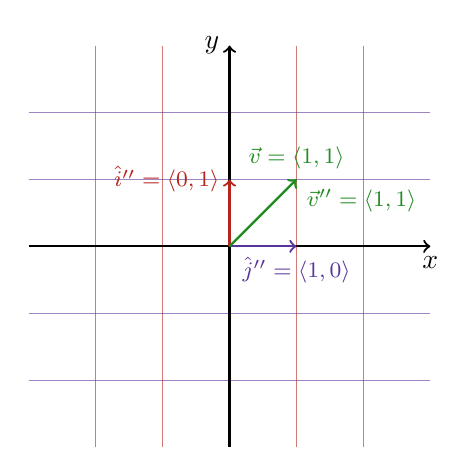
\begin{tikzpicture}[
        vector/.style={->, thick},
        scale=0.85
    ]

    \foreach \i in {-2, -1, ..., 2} {
        \draw[BrickRed, thin, opacity=0.6] (\i, -3) -- (\i, 3);
        \draw[RoyalPurple, thin, opacity=0.6] (-3, \i) -- (3, \i);
    }
    \draw[vector, black] (-3, 0) -- (3, 0) node[below] {$x$};
    \draw[vector, black] (0, -3) -- (0, 3) node[left] {$y$};

    \draw[vector, BrickRed] (0, 0) -- (0, 1)
        node[left, BrickRed]
            {\footnotesize $\hat{i}'' = \langle 0, 1 \rangle$};
    \draw[vector, RoyalPurple] (0, 0) -- (1, 0)
        node[below, RoyalPurple]
            {\footnotesize $\hat{j}'' = \langle 1, 0 \rangle$};
    \draw[vector, ForestGreen] (0, 0) -- (1, 1)
        node[above, dotted, ForestGreen]
            {\footnotesize $\vec{v} = \langle 1, 1 \rangle$};
    \draw[vector, ForestGreen] (0, 0) -- (1, 1)
        node[below right, ForestGreen]
            {\footnotesize $\vec{v}'' = \langle 1, 1 \rangle$};
\end{tikzpicture}
\end{figure}
\end{minipage}
\hfill
\begin{minipage}{0.48\textwidth}
\begin{figure}[H]
\centering
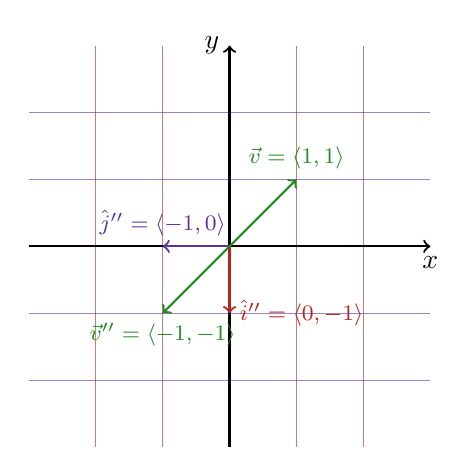
\begin{tikzpicture}[
        vector/.style={->, thick},
        scale=0.85
    ]

    \foreach \i in {-2, -1, ..., 2} {
        \draw[BrickRed, thin, opacity=0.6] (\i, -3) -- (\i, 3);
        \draw[RoyalPurple, thin, opacity=0.6] (-3, \i) -- (3, \i);
    }
    \draw[vector, black] (-3, 0) -- (3, 0) node[below] {$x$};
    \draw[vector, black] (0, -3) -- (0, 3) node[left] {$y$};

    \draw[vector, BrickRed] (0, 0) -- (0, -1)
        node[right, BrickRed]
            {\footnotesize $\hat{i}'' = \langle 0, -1 \rangle$};
    \draw[vector, RoyalPurple] (0, 0) -- (-1, 0)
        node[above, RoyalPurple]
            {\footnotesize $\hat{j}'' = \langle -1, 0 \rangle$};
    \draw[vector, ForestGreen] (0, 0) -- (1, 1)
        node[above, dotted, ForestGreen]
            {\footnotesize $\vec{v} = \langle 1, 1 \rangle$};
    \draw[vector, ForestGreen] (0, 0) -- (-1, -1)
        node[below, ForestGreen]
            {\footnotesize $\vec{v}'' = \langle -1, -1 \rangle$};
\end{tikzpicture}
\end{figure}
\end{minipage}

Let's take a look at what's happening here. $\vec{v}''$ in our
left diagram can be represented as the following.
\[
\vec{v}'' =
\begin{bmatrix}
    -1 & 0 \\
    0  & 1
\end{bmatrix}
\left(
\begin{bmatrix}
    0 & -1 \\
    1 & 0
\end{bmatrix}
\begin{bmatrix}
    1 \\
    1
\end{bmatrix}
\right)
\]
Notice that we have to write it in the order $B(A\vec{v})$ as we
would be performing $A$ first. We can think of it as reading it from
left to right just as we would read from left to right when
computing composite functions.
\[
\vec{v}'' =
\begin{bmatrix}
    -1 & 0 \\
    0  & 1
\end{bmatrix}
\left(
\begin{bmatrix}
    0 & -1 \\
    1 & 0
\end{bmatrix}
\begin{bmatrix}
    1 \\
    1
\end{bmatrix}
\right)
=
\begin{bmatrix}
    -1 & 0 \\
    0  & 1
\end{bmatrix}
\left(
\begin{bmatrix}
    -1 \\
    1
\end{bmatrix}
\right)
=
\begin{bmatrix}
    1 \\
    1
\end{bmatrix}
\]
This is exactly what we have for the left diagram. We could do
the same for the right side.
\[
\vec{v}'' =
\begin{bmatrix}
    0 & -1 \\
    1 & 0
\end{bmatrix}
\left(
\begin{bmatrix}
    -1 & 0 \\
    0  & 1
\end{bmatrix}
\begin{bmatrix}
    1 \\
    1
\end{bmatrix}
\right)
=
\begin{bmatrix}
    0 & -1 \\
    1 & 0
\end{bmatrix}
\left(
\begin{bmatrix}
    -1 \\
    1
\end{bmatrix}
\right)
=
\begin{bmatrix}
    -1 \\
    -1
\end{bmatrix}
\]
This is also supported! Alternatively, we could just compute
$AB$ and $BA$ to see what our ``final transformation is''.
\begin{align*}
    BA &=
    \begin{bmatrix}
        -1 & 0 \\
        0  & 1
    \end{bmatrix}
    \begin{bmatrix}
        0 & -1 \\
        1 & 0
    \end{bmatrix}
    =
    \begin{bmatrix}
        0 & 1 \\
        1 & 0
    \end{bmatrix} \\
    AB &=
    \begin{bmatrix}
        0 & -1 \\
        1 & 0
    \end{bmatrix}
    \begin{bmatrix}
        -1 & 0 \\
        0  & 1
    \end{bmatrix}
    =
    \begin{bmatrix}
        0  & -1 \\
        -1 & 0
    \end{bmatrix}
\end{align*}
Clearly, we could see that the mapping is different.

Another interesting property for matrices $A$, $B$, and $C$ is that
even if $AC = BC$, it does not necessarily mean that $A = B$.
Think about the case when $C$ is a zero matrix. Although matrix
multiplication is not commutative, the associative and distributive
property still applies.

\begin{theorem}{}{Properties of Matrix Multiplication}
For matrices $A$, $B$, and $C$, the following equations are true
given that the conditions for the addition and multiplication are met.
\begin{enumerate}
\item $A(BC) = (AB)C$
\item $A(B + C) = AB + AC$
\item $(B + C)A = BA + CA$
\item $\lambda(AB) = A(\lambda B)$
\end{enumerate}
\end{theorem}

Let's start by proving the associative property.
\begin{proof}
Let $A = [a_{ij}]_{m \times n}$, $B = [b_{ij}]_{n \times q}$,
and $C = [c_{ij}]_{q \times r}$. First, notice that the elements
of the product $BC$, or $D = [d_{ij}]_{n \times r}$ can be
represented as $d_{ij} = \sum_{k=1}^{q} b_{ik} c_{kj}$. Multiplying
it again with $[a_{ij}]$, the elements of the product
$E = [e_{ij}]_{m \times r}$ can be represented as the following.
\[
e_{ij}
= \sum_{s=1}^{n} a_{is} d_{sj}
= \sum_{s=1}^{n} \left(
    a_{is} \sum_{k=1}^{q} b_{sk} c_{kj}
\right)
= \sum_{s=1}^{n} \sum_{k=1}^{q} a_{is} b_{sk} c_{kj}
\]
Similarly, we could do the same for the right-hand side of the
equation. Note that the elements of the product $AB$, or
$D' = [d'_{ij}]_{m \times q}$ can be represented as
$d'_{ij} = \sum_{k=1}^{n} a_{ik} b_{kj}$. Continuing, the elements
in the final product $E' = [e'_{ij}]_{m \times r}$ can be written as
the following.
\begin{align*}
    e'_{ij}
    &= \sum_{s=1}^{q} d'_{is} c_{sj}
    = \sum_{s=1}^{q} \left(
        \left(\sum_{k=1}^{n} a_{ik} b_{ks} \right) c_{sj}
    \right)
    = \sum_{s=1}^{q} \sum_{k=1}^{n} a_{ik} b_{ks} c_{sj} \\
    &= \sum_{k=1}^{q} \sum_{s=1}^{n} a_{is} b_{sk} c_{kj}
    = \sum_{s=1}^{n} \sum_{k=1}^{q} a_{is} b_{sk} c_{kj}
    = e_{ij}
\end{align*}
Because $e_{ij} = e'_{ij}$ for all possible combinations,
$A(BC) = (AB)C$.
\end{proof}
\begin{thoughts}
You might wonder if we are allowed to say that the following equation
is true.
\[
\sum_{k=1}^{q} \sum_{s=1}^{n} a_{is} b_{sk} c_{kj}
= \sum_{s=1}^{n} \sum_{k=1}^{q} a_{is} b_{sk} c_{kj}
\]
When proving this property, I initially thought that my proof
contained an error and spent my time reading the proof over and
over again. This actually applies and visualizing it helped me.
This part is not rigorous, so I didn't include it in the proof
above, but you can think of rotating the entire summation by
$90^\circ$.
\[
\sum_{k=1}^{q} \sum_{s=1}^{n} a_{is} b_{sk} c_{kj}
=
\begin{array}{ccc}
    a_{i1}b_{11}c_{1j} & & a_{i1}b_{1q}c_{qj} \\
    \vdots & + \cdots + & \vdots \\
    a_{in}b_{n1}c_{1j} & & a_{in}b_{nq}c_{qj}
\end{array}
\]
Similarly, the second sum can be represented as the following.
\[
\sum_{s=1}^{n} \sum_{k=1}^{q} a_{is} b_{sk} c_{kj}
=
\begin{array}{ccc}
    a_{i1}b_{11}c_{1j} & & a_{in}b_{n1}c_{1j} \\
    \vdots & + \cdots + & \vdots \\
    a_{i1}b_{1q}c_{qj} & & a_{in}b_{nq}c_{qj}
\end{array}
\]
Now imagine you write the entire terms out, and rotate it
$90^\circ$. They are identical!
\end{thoughts}

Next, let's prove the first distributive law.

\begin{proof}
Let $A = [a_{ij}]_{m \times n}$, $B = [b_{ij}]_{n \times q}$,
and $C = [c_{ij}]_{n \times q}$. Consider the following equation.
\begin{align*}
    [a_{ij}] \left( [b_{ij}] + [c_{ij}] \right)
    &= [a_{ij}] [b_{ij} + c_{ij}]
    = \left[ \sum_{k=1}^{n} a_{ik} (b_{kj} + c_{kj}) \right] \\
    &= \left[
        \sum_{k=1}^{n} a_{ik} b_{kj} + \sum_{k=1}^{n} a_{ik} c_{kj}
    \right]
    = \left[ \sum_{k=1}^{n} a_{ik} b_{kj} \right]
        + \left[ \sum_{k=1}^{n} a_{ik} c_{kj} \right] \\
    &= [a_{ij}] [b_{ij}] + [a_{ij}] [c_{ij}]
\end{align*}
Therefore, the distributive property $A(B + C) = AB + AC$ applies.
\end{proof}

We could prove the right distributive law in similar fashion.

\begin{proof}
Let $A = [a_{ij}]_{n \times q}$, $B = [b_{ij}]_{m \times n}$,
and $C = [c_{ij}]_{m \times n}$. Consider the following equation.
\begin{align*}
    \left( [b_{ij}] + [c_{ij}] \right) [a_{ij}]
    &= [b_{ij} + c_{ij}] [a_{ij}]
    = \left[ \sum_{k=1}^{n} (b_{ik} + c_{ik}) a_{kj} \right] \\
    &= \left[
        \sum_{k=1}^{n} b_{ik} a_{kj} + \sum_{k=1}^{n} c_{ik} a_{kj}
    \right]
    = \left[ \sum_{k=1}^{n} b_{ik} a_{kj} \right]
        + \left[ \sum_{k=1}^{n} c_{ik} a_{kj} \right] \\
    &= [b_{ij}] [a_{ij}] + [c_{ij}] [a_{ij}]
\end{align*}
Thus, the right distributive property $(B + C)A = BA + CA$ holds.
\end{proof}

Finally, let's prove the fourth property.

\begin{proof}
Let $A = [a_{ij}]_{m \times n}$ and $B = [b_{ij}]_{n \times p}$.
Consider the following equation.
\[
\lambda (AB)
= \lambda \left[ \sum_{k = 1}^{n} a_{ik} b_{kj} \right]
= \left[ \sum_{k = 1}^{n} \lambda a_{ik} b_{kj} \right]
= \left[ \sum_{k = 1}^{n} a_{ik} (\lambda b_{kj}) \right]
= A(\lambda B)
\]
Thus, the fourth property holds.
\end{proof}

In addition to the visual implications of a matrix and its
multiplication above, matrix multiplication can be extended to
systems of equations. For instance, consider the following system
of equations.
\begin{align*}
    2x + 3y &= 5 \\
    -x + 7y &= 3
\end{align*}
Using \textbf{coefficient matrix}, we could represent the system
above as the following matrix multiplication.
\[
\begin{bmatrix}
    2  & 3 \\
    -1 & 7
\end{bmatrix}
\begin{bmatrix}
    x \\
    y
\end{bmatrix}
=
\begin{bmatrix}
    5 \\
    3
\end{bmatrix}
\]
Let's take a look at more interesting facts on matrix multiplication.

\begin{definition}{}{}
A square matrix with $1$ in all entries of its main diagonal and
$0$ in the other entries is an \textbf{identity matrix}, denoted as
$I_n$ for an identity matrix with order $n \times n$. Moreover,
all identity matrices satisfy the following equation for square
matrix $A$ that can be multiplied.
\[
AI = IA = A
\]
\end{definition}

This is called an identity matrix because when you multiply any
square matrix by the identity matrix with the corresponding order,
you get the square matrix itself. Consider the following examples.
\[
\begin{bmatrix}
    1 & 0 & 0 \\
    0 & 1 & 0 \\
    0 & 0 & 1
\end{bmatrix}
\begin{bmatrix}
    1 & 2 & 3 \\
    4 & 5 & 6 \\
    7 & 8 & 9
\end{bmatrix}
=
\begin{bmatrix}
    1 & 2 & 3 \\
    4 & 5 & 6 \\
    7 & 8 & 9
\end{bmatrix}
\]
From this, we can obtain an important fact about the uniqueness
of the identity matrix.

\begin{theorem}{}{Uniqueness of Identity Matrices}
The identity matrix $I$ for square matrices $A$ is unique.
\end{theorem}
\begin{proof}
For the sake of contradiction, let matrix $A_{m \times m}$ have two
unique identity matrices $I_{m \times m}$ and $J_{m \times m}$.
By definition, $AI = IA = A$ and $AJ = JA = A$. Therefore,
$AI = IA = AJ = JA$ and $AI = AJ$. Because $A$ is any square matrix
with order $m \times m$, let $A = I$. Substituting, $II = IJ$, and
$I = J$ is obtained by definition. By contradiction from the
assumption that $I \neq J$, the identity matrix for a square matrix
$A$ is unique.
\end{proof}

Another interesting insight on matrix multiplication is dissecting
the matrices being multiplied. Let's take a look at a simple example.
\begin{align*}
\begin{bmatrix}
    a_{11} & a_{12} & a_{13} \\
    a_{21} & a_{22} & a_{23}
\end{bmatrix}
&\begin{bmatrix}
    b_{11} & b_{12} \\
    b_{21} & b_{22} \\
    b_{31} & b_{32}
\end{bmatrix}
=
\begin{bmatrix}
    a_{11} b_{11} + a_{12} b_{21} + a_{13} b_{31} &
    a_{11} b_{12} + a_{12} b_{22} + a_{13} b_{32} \\
    a_{21} b_{11} + a_{22} b_{21} + a_{23} b_{31} &
    a_{21} b_{12} + a_{22} b_{22} + a_{23} b_{32}
\end{bmatrix} \\
&=
\begin{bmatrix}
    a_{11} & a_{12} & a_{13} \\
    0      & 0      & 0
\end{bmatrix}
\begin{bmatrix}
    b_{11} & b_{12} \\
    b_{21} & b_{22} \\
    b_{31} & b_{32}
\end{bmatrix}
+
\begin{bmatrix}
    0      & 0      & 0 \\
    a_{21} & a_{22} & a_{23}
\end{bmatrix}
\begin{bmatrix}
    b_{11} & b_{12} \\
    b_{21} & b_{22} \\
    b_{31} & b_{32}
\end{bmatrix} \\
&=
\begin{bmatrix}
    a_{11} & a_{12} & a_{13} \\
    a_{21} & a_{22} & a_{23}
\end{bmatrix}
\begin{bmatrix}
    b_{11} & 0 \\
    b_{21} & 0 \\
    b_{31} & 0
\end{bmatrix}
+
\begin{bmatrix}
    a_{11} & a_{12} & a_{13} \\
    a_{21} & a_{22} & a_{23}
\end{bmatrix}
\begin{bmatrix}
    0 & b_{12} \\
    0 & b_{22} \\
    0 & b_{32}
\end{bmatrix}
\end{align*}
In the matrix multiplication above, we could see that to find
the element in the entry $(i, j)$, it is sufficient for us to
see row $i$ from the left matrix and column $j$ from the right.
In the next section of the note, we will discuss different
topics about matrix.

\end{document}


